% Andrew G. West - prop_spec.tex
% Main LaTeX file for CIS400/401 Project Proposal Specification
%

\documentclass{sig-alternate}
 
\usepackage{mdwlist}
\usepackage{url}
\usepackage{graphicx}
\usepackage{float}
\usepackage[section]{placeins}
\begin{document} 

\title{PROTOS: A PR2 Open Tele-Operation System}

\subtitle{Dept. of CIS - Senior Design 2011-2012}
\numberofauthors{3}
\author{
\alignauthor Seth Shannin \\ \email{sshannin@seas.upenn.edu} \\ Univ. of Pennsylvania \\ Philadelphia, PA
\alignauthor Kevin Xu \\ \email{kevinxu@seas.upenn.edu} \\ Univ. of Pennsylvania \\ Philadelphia, PA
\alignauthor Dr. Camillo Jose Taylor \\ \email{cjtaylor@cis.upenn.edu} \\ Univ. of Pennsylvania \\ Philadelphia, PA}
\date{}
\maketitle

\begin{abstract}
\textit{\indent Programming a robot to autonomously perform human tasks has been a 
long-time goal of robotics. Such endeavors have typically involved heavy 
computation due to the demands of visual data processing, path planning, and motor 
coordination. One alternative to these computationally-intense methods is to use 
human demonstration to introduce a sequence 
of moves to a robot. This has been attempted
through both kinesthetic teaching (teaching via direct physical 
manipulation of the robot's limbs) and visual observation. Another way to teach through demonstration
can potentially be achieved by the development of an immersive
teleoperation system for controlling humanoid robots. Building on previous attempts to
control the PR2 from a distance (`teleoperation'), the system also aims provide the
operator with an `immersive' experience by providing a view of 
the environment from the robot's perspective.}

\textit{\indent The effectiveness of the system will be tested and evaluated by its ability to allow a human operator
to perform simple manipulation tasks with the robot, such as picking up a cup.
Following the implementation of this system, its performanced will be evaluated in two ways: the ease with which
a human operator can perform a given task, and the accuracy with which the system can record
the operator's movements and replay them faithfully at a later time.
If successful, the immersive teleoperation system will present a novel and natural method for a
human operator to demonstrate a specific movement sequence to a humanoid robot.}
\end{abstract}

\section{Introduction}
\label{sec:intro}
\subsection{Background}
\indent Constructing a fully autonomous and adaptive robot is one of the more
elusive goals of robotics research.
The possibility of a robotic butler is only one of many potential applications.
However, true autonomous decision making (that is, behavior free of direct 
control from a human operator) is an incredibly challenging process since many 
different systems must 
be coordinated to make this possible. Visual information must be processed 
quickly and accurately to respond to changes in the environment in a timely
manner. Robots also need accurate path planning to navigate their environment,
 and precise motor coordination to manipulate objects in the environment. 
 There have been many different attempts at overcoming these challenges 
involved in developing an autonomous robot.

\indent One major type of approach 
that has been often explored involves the field of machine learning. The ability to learn can be a powerful intermediate 
step towards autonomy, since learning can allow a robot to adapt to new, unforeseen scenarios on its own. 
Teaching by human demonstration is a common approach to robot learning because it enables the 
transmission of complex behavior in a manner far easier than individually planning the movement of each motor and joint. However, choosing exactly how the demonstrated behavior is delivered to the robot in such a way that it can record and reproduce that behavior is still a very challenging task.

\subsection{Approach}
\indent The {\tt PROTOS} system is designed to be an immersive teleoperation system for controlling the WillowGarage PR2 humanoid robot. `Teleoperation' means controlling the PR2 from
a distance. `Immersive', means giving the human operator the illusion of being inside the PR2.

\indent The PR2 is a humanoid robot developed by  Willow Garage~\cite{pr2} for the purpose of robotics 
research. It is omnidirectional and capable of telescoping height. The PR2 has a pair of highly movable arms and grippers
that allow grasping of many different kinds of objects. The PR2 also comes with a robust set of highly useful software development tools,
including a versatile simulator that allows developers to perform trial runs on a virtual PR2 without
risking damage to the actual robot or environment. Institutions across the
world have taught the PR2 a wide variety of human actions, such as baking 
cookies~\cite{cookies}, scanning and bagging groceries~\cite{groceries}, and fetching a sandwich~\cite{subway}.
 However, unlike in these examples, the proposed {\tt PROTOS} system will ideally enable the PR2 to acquire new behavior not through advanced task planning,
but rather through human demonstration. Thanks to the University of Pennsylvania's GRASP Laboratory, a real PR2 (shown in Figure~\ref{fig:pr2_photo}) can be used to test the
system implementation.

\begin{figure}[htb] 
	\begin{center}
		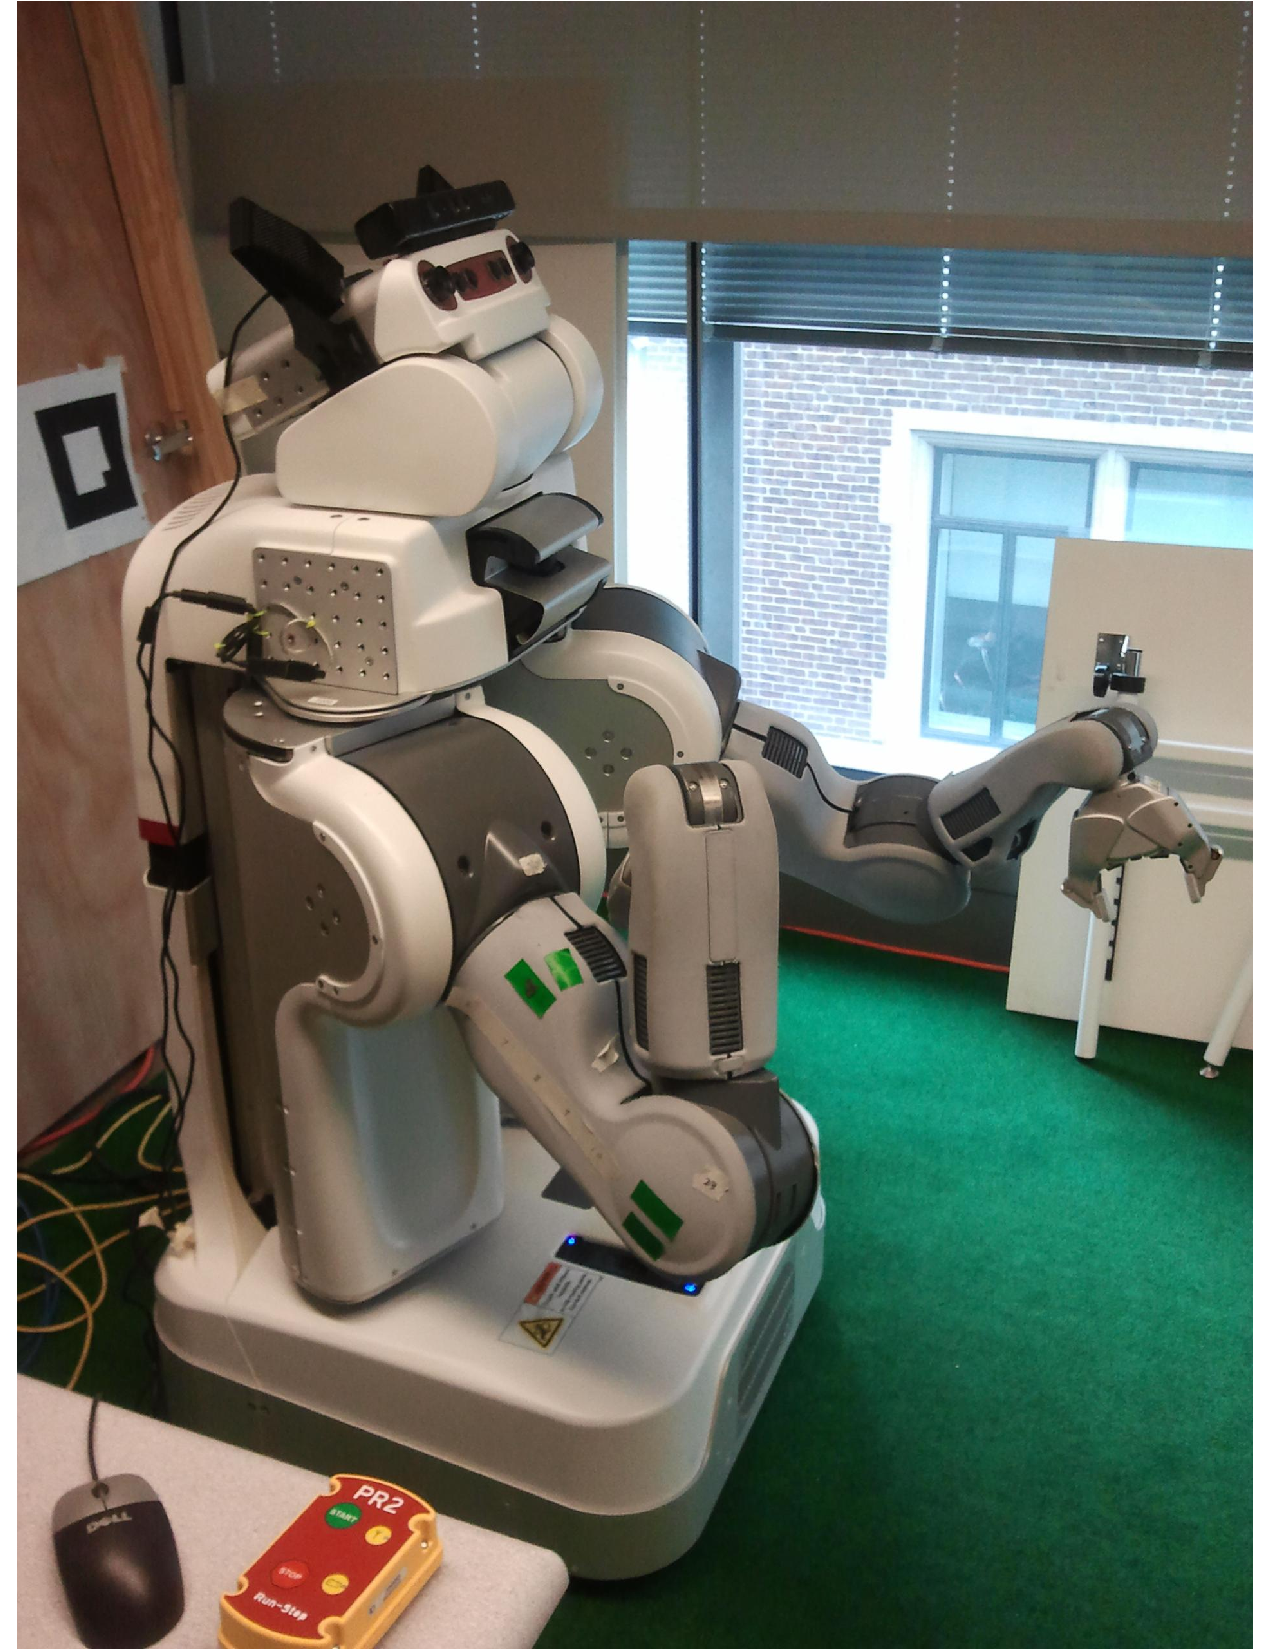
\includegraphics[width=0.8\linewidth]{graspy}
	\end{center}
	%\vspace{-24pt}
	\caption{PR2 robot at the University of Pennsylvania, nicknamed `GRASPY'}
	\label{fig:pr2_photo}
\end{figure}

\indent The chief component of the {\tt PROTOS} teleoperation system is the Microsoft XBox Kinect sensor. This sensor provides depth information at real-time speeds
(30 frames per second), also performing the computation that would have been required for stereo 
processing. Combined with various open source libraries~\cite{kinect}, the Kinect also works with 
software that provides human motion sensing and tracking, greatly simplifying the task of capturing human body movements.

\indent The Kinect will be used as part of an immersive teleoperation system to allow a human operator to easily demonstrate sequences of actions
to a PR2.
The Kinect sensor provides a convenient way to capture the human operator performing the desired behavior. The captured data can be relayed to the
PR2 via ROS, the open-source Robot Operating System~\cite{ros}. ROS provides a 
convenient framework for device abstraction, inter-process communication, and message recording.
By using ROS along with the PR2 and the Kinect, the {\tt PROTOS} system will allow remote operation of the PR2 while
allowing the operator to see the PR2's surroundings from the PR2's onboard cameras. The effectiveness of this system in performing simple tasks with the PR2 
was then evaluated.

\subsection{Results}
\indent The {\tt PROTOS} system was tested by having the human operator attempt to pick up a cup with the PR2. The PR2 was able to successfully pick up a cup and 
place it back down in its original starting location. This motion was also successfully recorded, and was able to be played back later without the help of a human operator.
The cup pick and drop motion was replayed fifteen times in succession before the PR2 finally failed to pick up the cup again, as the cup was knocked slightly out of
the PR2's reach.

\subsection{Organization}
\indent What follows is an overview of other work related to implementation of 
teleoperation systems and teaching robots human-like tasks (Section~\ref{sec:related_work}). We then describe 
the components of the immersive teleoperation system (Section~\ref{sec:system_model}) before delving 
into the technical implementation of each component (Section~\ref{sec:system_implementation}). What follows is an 
evaluation of results obtained from the {\tt PROTOS} system (Section~\ref{sec:results}) and a description of future work to be
done on the system (Section~\ref{sec:future_work}) The remainder of the paper deals with the ethics involved in using an immersive teleoperation
system (Section~\ref{sec:ethics}) and summarizes the conclusions drawn from implementing and testing the system (Section~\ref{sec:conclusions}).

\section{Related Work}
\label{sec:related_work}
\indent  Related work will now be discussed. First, work releated to teleoperation (Section~\ref{sec:teleop}) will be presented in general, followed by a look at
autonomous robots (Section~\ref{sec:autobots}) and teaching the PR2 (Section~\ref{sec:teach_pr2}). The section concludes with an analysis of different teaching methods 
by demonstration (Section~\ref{sec:demo_teach}).

\subsection{Teleoperation}
\label{sec:teleop}
\indent There have been many previous teleoperation implementations for robotic systems. Kofman \textit{et al.}~\cite{robot_interface} devised a teleimmersive system for
controlling a robotic arm via teleoperation and sending visual feedback to the user. The setup used in their work involves multiple cameras aimed at the human operator to 
capture 3-D information about the operator's arm movements. This data is then sent to a remote site containing the robotic arm and mapped to its joints so it can mimic the 
motion of the human arm. The human operator is able to see the robotic arm via cameras positioned at the remote site that send visual feeds of both the entire arm and of 
vision from the point of view of the tip of the robotic arm. Fortunately, the Kinect, when paired with ROS, provides a much simpler and cost efficient setup to 
capture arm motion and transmit data to the PR2. The Kinect requires almost no work to setup, and can be purchased at little cost compared to a complex motion capture setup
involving multiple cameras. Willow Garage has already 
tried integrating Kinect with ROS to control the PR2 remotely~\cite{willow_kinect}. However, the {\tt PROTOS} system uses immersion as a tool to help the user teleoperate
the PR2, which is something that the Willow Garage implementaton appears to lack.

\subsection{Autonomous Robots}
\label{sec:autobots}
\indent A common approach to autonomous robot action relies primarily on heavy amounts of computation to carefully 
plan each action that the robot will execute ahead of time.  The chief 
advantage that the {\tt PROTOS} system intends to provide over these methods is that it 
not only serves as an immersive teleoperation system with which a robot can be used to
execute tasks, but also as a provider of demonstration data
that can be used to teach a robot to do these kinds
of things more quickly and naturally by using data from a human operator using the 
teleoperation system execute the actions.

\indent Other institutions have conducted research involving autonomous robots handling
drinks. Hillenbrand \textit{et al.}~\cite{pouring_arm} designed a 
semi-autonomous hand-arm robot for this purpose. The hand-arm was capable of 
responding to user input by choosing a drink from a variety of different 
containers, opening the drink if necessary, pouring the liquid into a glass, 
and then offering the cup to the user. It was capable of not only picking up 
bottles and cups, but also of unscrewing bottle caps. Processing of visual data
from cameras was combined with object recognition to identify the drinks, after
which grasp planning was used to actually pick up and manipulate the drink.

\indent Srinivasa \textit{et al.}~\cite{herb} designed an autonomous robot capable of 
navigating a household-like environment and manipulating a wide variety of 
everyday objects. Consisting of an arm mounted on a segway, HERB used a 
powerful array of six multi-core processors to successfully traverse its 
environment and interact with objects around it, such as cups and drawers. By 
combining different processes for object recognition, task based planning, and 
caged grasping, HERB was able to autonomously carry out commands issued from a 
graphical user interface to perform simple kitchen tasks, such as placing an 
object in a recycling bin or lifting a mug.

\subsection{Teaching the PR2}
\label{sec:teach_pr2}
\indent Substantial work has been done in teaching the PR2 robot to perform various human tasks.  These approaches to teaching the PR2 emphasize complex algorithms used 
to enable the PR2 to devise a plan from scrach to act autonomously in a 
given environment.  Bohren \textit{et al.}~\cite{beer} used the PR2 and ROS to build a robotic 
system for retrieving beverages from a refrigerator. In their work, they developed a task-level execution system for rapidly prototyping different robotic applications. 
The PR2 had to navigate an obstacle map to reach the refrigerator, use object recognition and grasp planning to identify the door handle and the drinks, and ultimately use 
facial recognition to deliver the beverage to a human recipient. 
Klingbeil \textit{et al.}~\cite{groceries} developed a grasping algorithm to enable the PR2 to pick up objects and attempt to locate and scan the barcode. Their 
technique allowed the PR2 to devise a plan to grasp the object from only a single 3D snapshot.
Saito \textit{et al.}~\cite{subway} devised a way for the PR2 to intelligently 
navigate large environments via semantic search. The PR2 attempts to find a specific object by first searching areas that would logically contain that item.

\indent The {\tt PROTOS} system will hopefully simplify teaching methods by enabling use of recorded input data from immersive teleoperation to give the PR2 
a general sequence of actions  to follow that can later be refined through more complex learning techniques.

\subsection{Teaching by Demonstration}
\label{sec:demo_teach}
\indent Various approaches involving data from human demonstration have been explored to allow a robot to perform specific tasks. In a relatively early attempt, 
Chalodhorn \textit{et al.}~\cite{walk_imitation} used motion capture to teach a bipedal humanoid robot how to walk by imitation. Joint angles obtained from motion capture 
data recorded from a human demonstrator wearing a motion capture suit were mapped to joint angles on the robot.
Kormushev \textit{et al.}~\cite{whiteboard} taught a robot new motor skills through kinesthetic teaching, which is 
teaching by physical contact. The robot had two distinct modes of operation: a learning phase and a reproduction phase. First, the robot was shown how to clean a whiteboard 
by direct human manipulation of the robot's joints, recording both position and force information. Subsequently, the robot would translate the learned information to its own 
frame of reference and attempt to duplicate the teacher's movement pattern on the whiteboard.  Kormushev \textit{et al.}~\cite{pancakes} also used kinesthetic learning to 
teach a robotic arm how to flip a pancake. 
Reinforcement learning techniques were applied such that the robot could evaluate the performance of its flips and attempt to adjust the motion 
of the arm for better future flips.

\indent The {\tt PROTOS} system has several advantages over these existing approaches. First of all, the Kinect sensor provides accurate real-time human
motion tracking that can be mapped to specific movement in the PR2 thanks to ROS. The Kinect also provides motion capture without the need
of complicated setups involving motion capture suits or multiple cameras. Secondly, an immersive scheme for controlling the robot
enables a human operator to more naturally move the robot in a given situation,
especially compared to manipulating the robot directly by physical
contact or through a joystick-based control scheme. Immersive teleoperation also enables direct control of robots that cannot be easily
subject to demonstration through physical contact, such as very large or very small robots. This sytem, if successful, would allow for rapid demonstration of different 
sequences of behavior to the PR2, which could be stored and queued up for later reproduction and enhancement. This technique could be generalized to other humanoid robots 
besides the PR2 to teach them different kinds of behavior. Any humanoid robot could potentially be controlled with {\tt PROTOS} with relatively minor modification to the source code.
The tasks also need not be restricted to lifting simple objects, as the system can capture data from the human user's entire body.

\section{System Model}
\label{sec:system_model}
Because a teleimmersive system is meant to be used by a human 
operator to control a robot, the external/visible part of this
design must be simple. The number of devices used to get input from the user 
and to deliver feedback should be small, and these devices should require
minimal effort to use. To that
end, a good portion of the control data captured from the user is captured
passively. After the initial setup phase, the user should be able to control
the system with minimal effort; the system should just watch the user and
translate the user's movements into control instructions for the PR2.

To facilitate this process, a few separate devices and some
fairly sophisticated software stacks were used. These devices will be discussed
in the upcoming section. The chief component of the system is the PR2 robot (Section~\ref{sec:model_PR2}) that
the user controls. ROS (Section~\ref{sec:model_ros}) is the component responsible for interfacing with devices and coordinating all the pieces of the
{\tt PROTOS} system by passing data between them as messages. While the
Microsoft Kinect is used to perform most of the motion capture, an additional
devices and accelerometers are needed to capture motions of the head and hands (Section~\ref{sec:model_motion}). 
In particular, there are a few button devices which allow the user to
perform non-humanoid operations on the robot (such as freezing a joint or
triggering certain actions capable only by the robot).

\subsection{PR2}
\label{sec:model_PR2}
The most obvious component of the system is the actual PR2 robot. This is the
device that user will control through teleimmersive operation. The user must
be able to control each of the PR2's motors, including those for the head,
arms, hands, gripper, torso, and base of the robot. To make the teleoperation
immersive, the user will need to receive a direct feed from the PR2's onboard
camera system.

\begin{figure}[htb] 
	\begin{center}
		\includegraphics[width=0.8\linewidth]{block}
	\end{center}
	%\vspace{-24pt}
	\caption{Block diagram summarizing system model}
	\label{fig:some_graph}
\end{figure}

\subsection{ROS}
\label{sec:model_ros}
While the PR2 may be the most apparent aspect of the system,
the true nexus is ROS, the Robot Operating System. Although the
user will never need to interact explicitly with ROS, all communication between
the user and the PR2 (in the form of commands or feedback) must pass through ROS.
ROS abstracts over devices and I/O, providing a common interface for accessing
any data stream or controlling any device. Processes that perform computation are visualized as nodes in a graph, with inter-process communication representing the
edges of the graph. Nodes send information to each other in the form of messages. Nodes that wish to send messages to other nodes can
`publish' to a topic, and nodes wishing to receive these messages need only to `subscribe' to these topics. ROS enables building relatively short
programs to issue surprisingly sophisticated commands to the PR2, such as moving all of the arm joints to a specific position within a
specified time frame.

By using ROS, the system can easily coordinate
data coming from the many tracking devices, process all this data and generate
movement plans for the PR2, and then send commands to make the PR2 to move in the
desired manner. This system architecture is shown Figure~\ref{fig:some_graph}.

\subsection{Motion Control}
\label{sec:model_motion}
Other than the PR2 robot itself, the Microsoft Kinect is perhaps the most 
prominent and important device in the teleimmersive operation system. ROS has 
existing Kinect libraries that allow
data from a Kinect to be handled as easily as any other message transmitted across the ROS network. A screenshot
of these libraries in action can be seen in Figure~\ref{fig:kinect_screenshot}.
These Kinect libraries have already been used successfully in 
many projects involving real-time tracking of human motion, examples of which can be found online~\cite{freenect}.
The hardware uses an 
infrared projector and stereo RGB cameras to create a 3D scene image complete
with depth information. It sends these raw video frames to ROS, which then
forwards the feed to a processing node. This processing node analyzes the 
video stream, identifies humanoid figures in the frames, and tracks these 
figures' joints. The Kinect does have some shortcomings in that it does 
not reliably track wrist, finger, or head movements. Separate 
accelerometer units are used to track these motions.

\begin{figure}[htb] 
	\begin{center}
		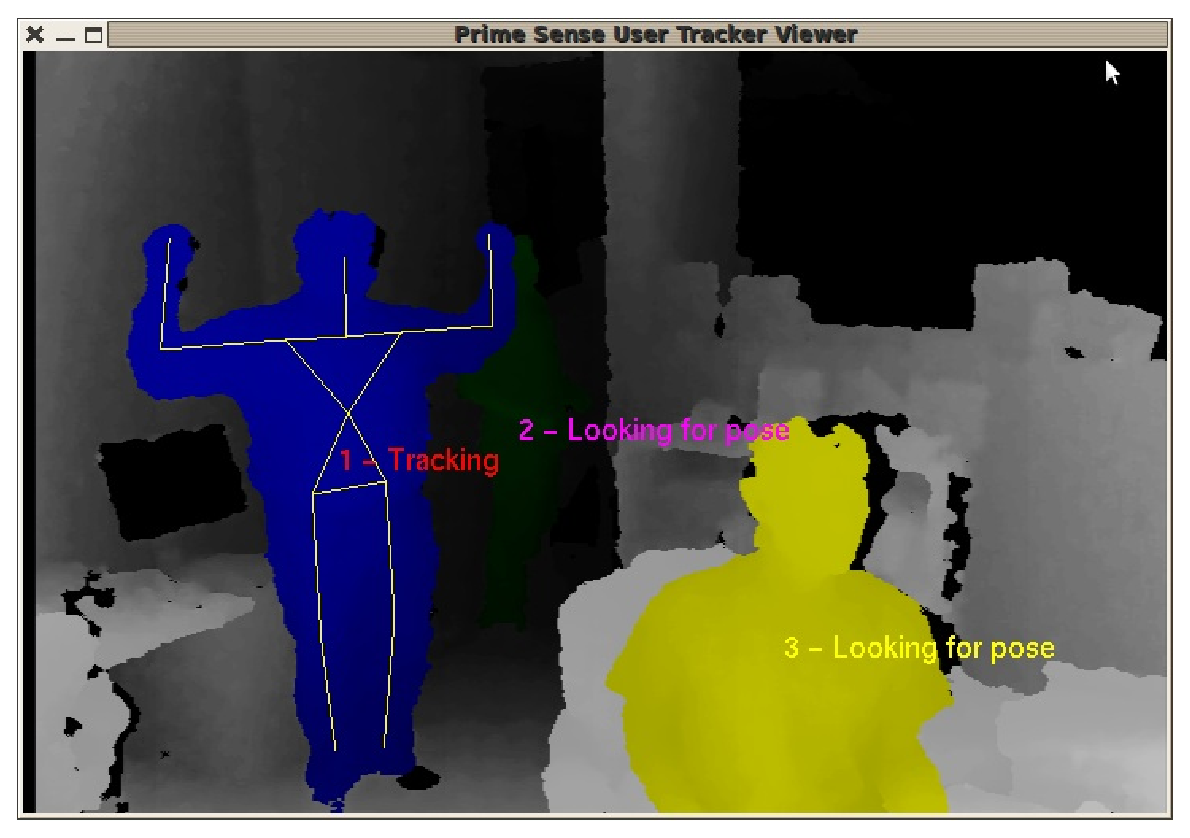
\includegraphics[width=0.8\linewidth]{kinect}
	\end{center}
	%\vspace{-24pt}
	\caption{Screenshot~\cite{kinect_pic} showing Kinect's tracking capabilities. The tracking software runs as a ROS node.}
	\label{fig:kinect_screenshot}
\end{figure}

\indent Wrist motion is captured by having the user hold one Nintendo Wiimote 
in each hand. The Wiimote is a video game controller with 
multiple buttons, a direction pad, and built-in accelerometers. 
The user can comfortably hold one Wiimote in each hand,
as this is how they were intended to be used in video games. and now has
convenient access to a number of
control buttons. These control buttons are used to perform a variety of actions
involving the PR2's wrists and grippers, such as opening/closing the grippers and
rotating/flexing the wrists. The remotes also carry accelerometers that could potentially be used
to track wrist movements. 

\indent In order to track the user's head movements, the user wears a hat
with an attached Intertial Measurement Unit (IMU) that acts as three-axis accelerometer. The IMU can track the yaw, pitch, and roll of the user's neck joint and can therefore relay all head motions to ROS. The device is
approximately the size of a quarter and can be attached to any surface via velcro or tape. This tracking of head movement is critical to the immersive aspect of the system
because it allows the PR2's head orientation to match that of the user's.
This ensures that the visual feedback shown to the user shifts accurately
as the user looks around the environment.

\subsection{Immersive Feedback}
\label{sec:model_feedback}
The final hardware device is a pair of Vuzix augmented reality glasses.
Essentially, this is a pair of glasses containing a mini LCD screen in place of
each lens. The glasses behave as
an external monitor that mirrors the video signal to both screens in front
of the user's eyes. 
The video feed from the PR2's wide-angle onboard camera is piped
directly into the glasses. This is the immersive step which closes the loop and
helps place the user more fully into the system. One technical limitation of the glasses is
the inability for the glasses to display true 3-D images to the user, since the same image is
shown on both lenses.

\subsection{Software}
\label{sec:model_software}
There is one other significant component to this system. This is the
component we have
termed in Figure~\ref{fig:some_graph} as the {\tt PROTOS Software}. This is a 
software node residing in ROS. Its primary function is to stitch together the
motion and position data from all the input devices (Kinect, Wiimotes, head 
IMU) and send commands to the robot. It processes all the information to map the user's motions
into equivalent motions for the PR2. The commands issued by the software can also be easily recorded by 
ROS and stored in a file. These files can be archived, and later replayed to cause the PR2 to repeat an action.
These stored actions can be played one after another to potentially chain together simpler actions into
more complex command sequences.

\section{System Implementation}
\label{sec:system_implementation}
Most of the interesting work in this project takes place inside the
{\tt PROTOS Software}, which aggregates all the captured motion data from the
user and processes this data to generate commands for the robot. ROS provides
bindings for both {\tt C++} and {\tt Python}. {\tt Python} was the language of choice due to avoid
the the relative verbosity of {\tt C++}.
The software runs as a node within ROS, and listens for interrupt events from the Wiimotes and head-mounted
IMU while actively polling for events from the Kinect. The events contain data
from these devices that report on the user's current actions and position. Figure~\ref{fig:human_model} shows
a human operator using the devices that comprise the {\tt PROTOS} system (minus the Kinect).

\begin{figure}[htb] 
	\begin{center}
		\includegraphics[width=0.8\linewidth]{pr2model}
	\end{center}
	%\vspace{-24pt}
	\caption{Photograph of a human operator using the {\tt PROTOS} system.}
	\label{fig:human_model}
\end{figure}

\subsection{Handling Kinect Input}
\indent ROS interfaces with the Kinect using the {\tt openni} Kinect software stack. The primary
function of this stack is to create a ROS node named {\tt openni\_tracker}. This
node identifies the Kinect device on a USB port and requests data
from it. It then attempts to identify people in the scene frame and start
tracking them. Once it has done so, it will publish data on various
topics (such as {\tt left\_shoulder}, {\tt right\_elbow}). These messages
contain joint angle transforms that are delivered to the {\tt PROTOS Software}.

\indent The {\tt PROTOS Software} receives messages from the
 {\tt openni\_tracker}.
When it receives information for an altered joint position, it applies the
appropriate transformations and instructs the PR2 on how to set its own joints
so as to mimic the sensed movement of the user. This is done for the shoulder
and elbow joints on both arms.

\subsection{Handling IMU Input}
\indent A similar process occurs for the IMU on the user's head (see Figure~\ref{fig:imu}). The specific IMU used in our system is
the CHR-6dm Attitude and Heading Reference System~\cite{imu_chr}. When lying flat, it uses its
accelerometers to capture roll and pitch. It also has a magnetic compass to 
track yaw (necessary since the plane in which the yaw rotational motion occurs
is perpendicular to the force of gravity). After connecting to the 
controlling computer via USB, a ROS node is run to read in data from the sensor and republish this data
encapsulated in ROS messages. The {\tt PROTOS Software} is notified when these
messages are published. It reads the roll, pitch, and yaw data in the message
and sends the appropriate commands to the PR2.

\indent The IMU must first be initialized before orientation information can be transmitted. Since the IMU uses a compass
to track yaw, values are reported as angular deviations from magnetic north.
Therefore, when tracking a user who does not begin by facing north, it is 
important to find the unity position for the sensor (the bearing when 
the user is facing forward) and to use this as an offset for all future angle
readings.

\begin{figure}[htb] 
	\begin{center}
		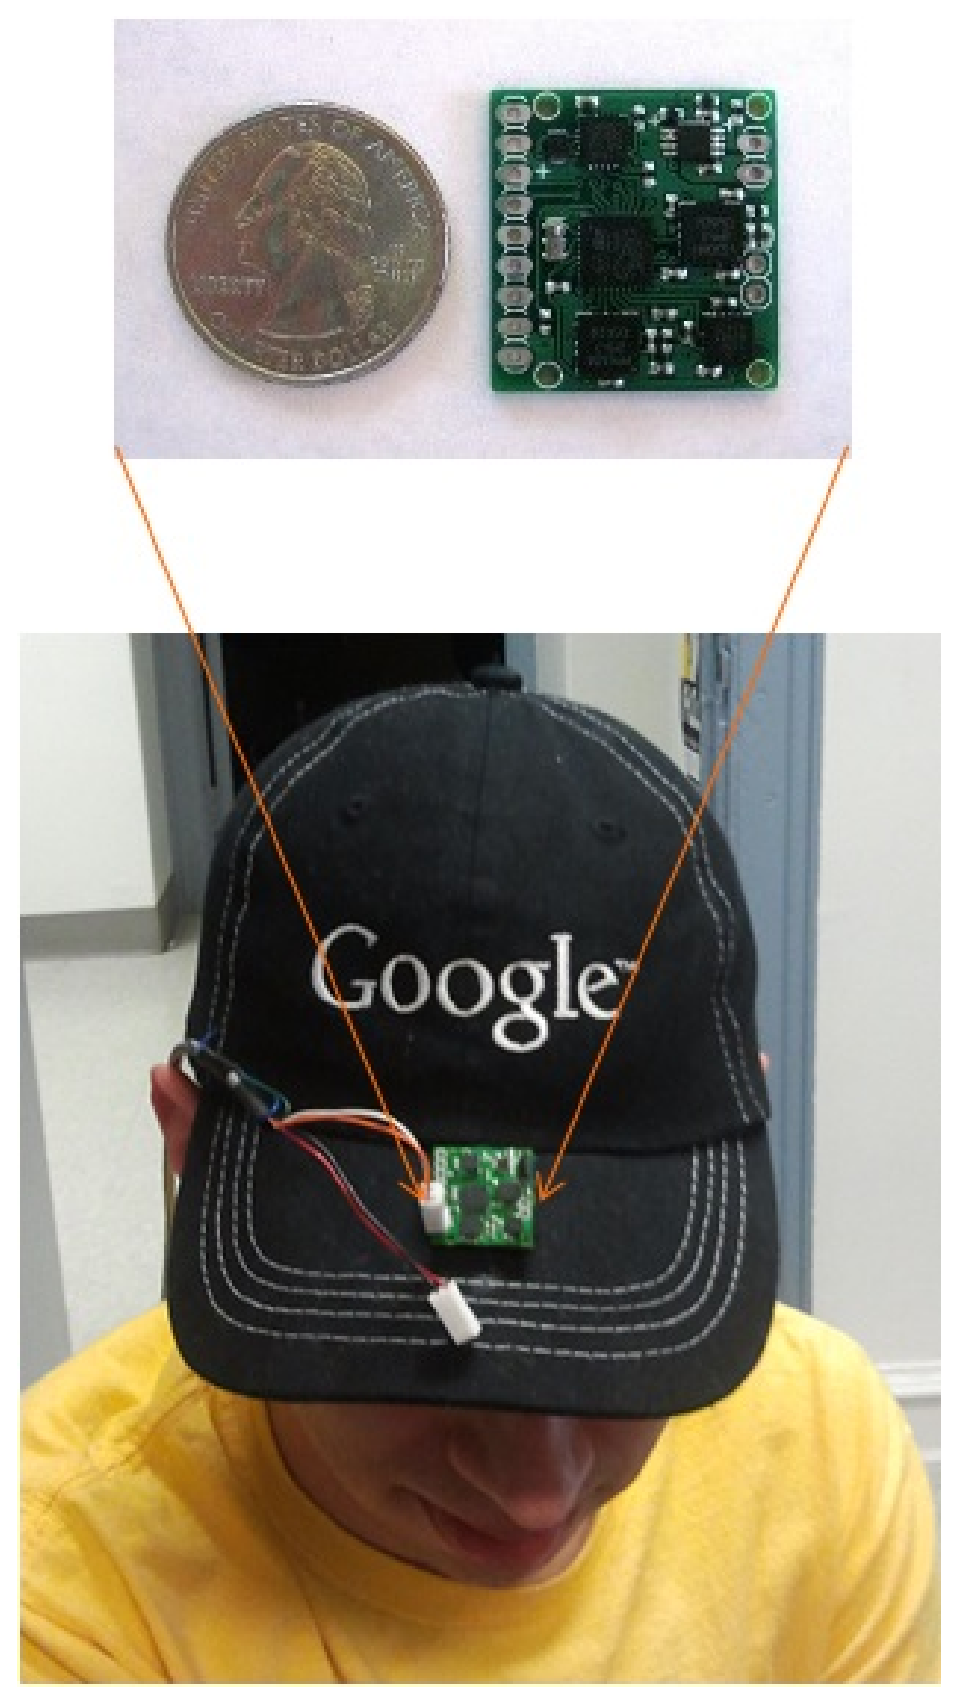
\includegraphics[width=0.6\linewidth]{imu}
	\end{center}
	%\vspace{-24pt}
	\caption{Photograph of a human operator wearing the IMU mounted on a cap.}
	\label{fig:imu}
\end{figure}

\subsection{Handling Wiimote Input}
The Wiimote communication is handled in much the same manner as the IMU on the head.
Instead of communicating via a USB port, however, the Wiimotes communicate wirelessly with the
controlling computer via Bluetooth. After the Wiimote pairs with the system,
ROS is used to create a Wiimote node which 
sends a periodic stream of messages. Each message is a vector containing the
status of each button and sensor readings from the Wiimote. The {\tt PROTOS Software}
listens for these messages. It notes the state of each button (whether or not that button
is pressed down)
and takes the appropriate action by sending commands to the PR2. 

\indent Additionally,  the {\tt PROTOS Software} can also read in accelerometer data from the Wiimote. The Wiimote
provides only the actual angular velocities; it doesn't not translate the 
values into roll, pitch, or yaw positions. Early builds of the system attempted to use these angular velocities along 
with the publishing frequency to compute an approximation of the actual roll, pitch,
and yaw angles of the human wrist. The angles were translated into the PR2's
reference frame, and commands were sent to instruct the PR2 to move its wrists accordingly. However,
this approach was ultimately sidelined in favor of using the Wiimote's buttons to control the PR2's
wrist and forearm movements. The translation process from the Wiimote's acceleration readings to the PR2's
wrist motions proved more difficult than anticipated due to the challenge in decoupling actual wrist movement
from more general arm movements.

\subsection{Physical Communication with the PR2}
\indent The physical method of
communication with the PR2 also merits discussion. One option was to have the PR2's onboard computers
act as the controllers for sending actions to the PR2. Since this is a teleimmersive operation system, this method is impractical, 
as the input devices used to capture human motion may not be physically located
near the PR2, thereby preventing the PR2's onboard computers from receiving data from these devices. 
In addition, it is impractical to attach all of these input devices 
directly to the PR2. This option was therefore ruled out early on in the implementation process. 

\indent The PR2 also contains multiple routers and hosts its
own wireless network. Therefore, remote communication with the PR2 became method of choice for interfacing
with the PR2 for the sake of simplicity. In a large scale, real world implementation of the {\tt PROTOS} system, however,
this manner of communication suffers from the same main issue as the first method - the user and devices
may be out of range of the WiFi source of the PR2. Fortunately,
the PR2 can also connect to other networks and aquire a public IP
(communicating either by WiFi or by
Ethernet). Although network complications have arisen when using this method,
these problems likely are due to issues with the computer used to run the system software 
rather than issues with the PR2's onboard routers.

\subsection{Visual Feedback}
\indent The final aspect of the system is the method used to relay visual feedback from the PR2 to the user.
A pair of  Vuzix virtual reality goggles is used to provide this feedback to the user. The PR2 sends multiple image 
streams to ROS from its multiple on-board cameras. As the goggles are not truly 3D, only one of the camera feeds
can be sent to the goggles. The images from the PR2's right head camera are sent to a node which displays the image
on the screen of the controlling computer. The video goggles can simply connect
to the VGA video out port of the computer to
receive the image and display it to the human operator. This video feed is sufficient
for performing simple tasks, but more complex ones will require some way to provide stereo vision feedback
to the user. A pair of goggles that contain true 3D capabilities that allow different images to be streamed
to the left and right lenses would be ideal.

\section{System Performance}
\label{sec:system_performance}
\indent The {\tt PROTOS} system has been evaluated both for its ability to correctly
imitate the actions of a human operator as well as for its potential 
to capture and reproduce useful data that can be used to aid demonstrative learning
attempts to allow the PR2 to acquire new behavior.

\subsection{Performance of Devices}
\indent The PR2 has lived up to its expectations as a good choice of humanoid robot to 
use as a target for the {\tt PROTOS} system. The 
PR2 is fully capable of all of the arm motions, head motions, and grasping
required for a variety of tasks, such as grasping simple objects. ROS has also been a superb framework that allows the 
{\tt PROTOS software} to easily communicate back and forth with the diverse 
assortment of devices that comprise the teleoperation system.

\indent  ROS makes receiving the data from the various devices incredibly simple. Capturing motion with the Kinect has been a painless process. 
The Kinect requires virtually no setup time and can transmit live human motion data in real time without the 
need for any special clothing or markers to indicate human joint locations.
The Wiimotes transmit their data wirelessly and accurately report button presses, rotations, and accelerations up to one hundred times per second. They fit 
nicely in the palms of the human operators' hands since they are originally intended to be used as video game controllers. The three-axis accelerometer for capturing head 
movement has worked very well in reporting the operator's head tilts and rotations.

\subsection {Performance of the {\tt PROTOS} Software}
\indent The performance of the {\tt PROTOS Software} has undergone numerous improvements since its conception. 
Although the physical devices that comprise the immersive teleoperation system 
are easy to use and are relatively few in number, the software has had an uneven performance history in translating data from these devices 
into appropriate actions for the PR2. The arm motion used to be very abrupt and prone to sudden, uneven movements. This lack of 
precision in movement maked it difficult for the human operator to precisely control the arms to the degree needed for fine motions such as lifting cups or glasses. This
issue was remedied in two ways. First, the software now smooths out the arm motion by threshholding the joint angles received from the Kinect.
This is done to essentially remove noise from the Kinect output picked up by unintentional arm shaking or wobbling. New actions are only sent to the PR2 if data received 
from the Kinect indicates that the operator's arms have moved a certain amount from their previous positions. Second, a reduction in the number of times per second that the
{\tt PROTOS Software} sends commands to the PR2 was reduced, which has improved performance in not only the arm movements, but the head movements as well. Sending the 
number of commands at a more reasonable rate (30 times per second, down from 60-100 per second) has greatly smoothed the PR2's movements, as the previous flood of commands
was causing the PR2's current goal to be interrupted, thus producing shaky movement.

\section{Results and Evaluation}
\label{sec:results}
The PROTOS system was evaluated based on two main criteria: its ability to allow a human operator to perform simple grasping tasks, and its ability to record said task
and replay it accurately at a later time. 

\subsection{Grasping Tasks}
\indent The performance of the {\tt PROTOS} immersive teleoperation system was first
evaluated based on how well it could translate actions of
the human operator to commands for the PR2. A human operator attempted to grasp a variety of cups and stuffed animal toys 
with the PR2 using the system. These small objects were placed near the PR2 on a raised surface (such as a desk or table), and the user was given the challenge of
picking that object up, moving it around in the air, and then placing the object back down in the same spot.

\indent Although the arms responded well to movements along the sides of the user, the movements became more
muddled when attempting to move in the area in front of the user's body. This is likely an artifact of the Kinect's inability to properly distinguish the operator's arm 
joint angles when they are bunched close together in front of the operator's body. Therefore, grasping objects directly in front of the PR2 was difficult, but grasping
objects to the side was still feasible. The Wiimotes responded well with no real hindrances to the grasping process. The buttons feel responsive and almost lagless in
transmitting directions to the PR2's grippers.

\indent The IMU was very responsive and provided accurate tracking of the human operator's head movements, which translated very well to the PR2's head movements. The user 
was able to keep the PR2's head mounted cameras focused on the object to be grasped. A framerate issue arose with the virtual reality goggles. Although the PR2's head movements
matched those of the user's, the rate at which images from the PR2's cameras were displayed to the goggles could not keep up with the rate at which new video was coming
in from the cameras. The user's view became choppy, which made grasping the objects more difficult. However, this issue can likely be remedied by simply using a more
powerful computer with which to run the {\tt PROTOS} system.

\subsection{Recording and Playback}
\indent Once the accuracy of the {\tt PROTOS} teleoperation system was improved, successful grasping trials were recorded by the {\tt PROTOS} system. ROS provides a very
convenient method for saving all messages that get transmitted by a ROS node. By using this mechanism, all of the commands issued by the {\tt PROTOS Software} to the PR2
can be stored in a file called a bagfile. These bagfiles can later be replayed to transmit the exact same sequence of commands to the PR2. The successful grasping trials
were replayed faithfully by the bagfile, and the PR2 was able to pick up the cup again without any outside help. However, the replay depends on the environment being setup
in exactly the same way as the time the recording was made. A depiction of the setup used for the recording and playback is pictured in Figure~\ref{fig:evaluation}. A cup
was placed on a desk next to the PR2. A human operator used the {\tt PROTOS} system to pick up the cup, move it around in the air, and then place it back down in the same location.
The entire process was recorded, and later played back without a human user involved. The PR2 was able to pick up the same cup and place it down fifteen consecutive times
before the cup was pushed out of the PR2's reach.

\indent The success of the recording and playback is promising for demonstration learning purposes, as motion sequences from the
 human operator can be recorded with a high degree of
accuracy. Any learning framework that can read in the rosbag files will be able to use these human sequences as demonstration data. The ease with which the {\tt PROTOS} system can 
produce these recordings makes it an ideal tool to augment a demonstration learning framework. The variety of motion sequences capable of being produced is not restricted
to only grasping, as any task involving the PR2's arms and head can be successfully performed and recorded.

\begin{figure}[htb] 
	\begin{center}
		\includegraphics[width=0.8\linewidth]{evaluation}
	\end{center}
	%\vspace{-24pt}
	\caption{The PR2 was able to continously pick up and place the same cup fifteen consecutive times by replaying data recorded from the {\tt PROTOS} system.}
	\label{fig:evaluation}
\end{figure}

\section{Future Work}
\label{sec:future_work} Perhaps the most obvious direction to pursue with
future work is the use of the recorded motion sequences as training data
for a machine learning-driven planner. Current planners can take multiple 
minutes to calculate even simple paths. Significant improvements in efficiency have 
already been demonstrated with planners using previously computed paths as a 
basis for new planning requests (the planner teaches itself)~\cite{mit_planning}. It would be
very interesting to explore training such a planner with recorded teleoperation
data from the PROTOS system, perhaps establishing more efficient and/or natural motions to serve as
a basis for future planning. For instance, by demonstrating a cup grasp with the PR2, the planner
could extrapolate based on one successful trial and enable the PR2 to autonomously grasp other cups
of similar size and shape.

\indent Another interesting avenue to pursue in the future would be to give the 
operator control over the movement of the PR2's base. Currently, only
the operator's head and arm movements are translated into PR2 commands. As the
Kinect also captures leg data, it is certainly possible to use different
motions or stances to instruct the PR2 to move in a certain direction.
Using actual walking motions would require sufficient space for both the PR2
and observation system however, while 
using stances would detract from the immersive aspect of the system. However,
if implemented, leg motion capture would open up many possibilities in terms of
motion sequences that could be imparted on to the PR2. The PROTOS system could 
command the PR2 to
nagivate hazardous environments, search a room for specific items, or deliver
objects from one point to another.

\section{Ethics}
\label{sec:ethics}All of the ethical considerations which apply to robotics in 
general are certainly still relevant when examining robotic teleoperation systems.
Also, there are two aspects of teleoperations systems which merit additional
consideration when evaulating these systems in terms of ethics. \\
\indent First and foremost, the behavior of the teleoperation system itself 
must be examined. It must be ensured that the system is accurate in its mimicry
of the operator in live settings, and that the system is precise when
recording commands for future playback. The level of trust required in the
accuracy of the system is clear; consider, for example robot-assisted surgery.
It is imperative that the PR2 not cause unintended harm to its environment, 
including the operator during training. To that end, it will be important
for the system to provide a mechanism that clearly segregates actions recorded 
under different scenario assumptions. As an example, the PR2 should not attempt to 
perform a physical handshake with a user while  in the middle of playing back a routine
for cutting vegetables. The teleoperation system should also
prevent actions which would stress the PR2's capabilities or otherwise
damage the PR2. The human operator could potentially harm the PR2 and its surrounding environment
with unnecessarily rapid movements and rigorous movements. Limits need to be placed on the PR2's
range of motion to ensure the safety of the operator, the PR2, and any other parties involved. \\
\indent Considering another aspect of the system, it is important to ensure
user accountability for actions performed with the PROTOS system. 
As the PR2 is primarily controlled via WiFi, it is important
to make sure that unauthorized individuals cannot send commands to (or 
otherwise control) the PR2. Any device which operates on a public IP should 
have safeguards in place, but this is especially important when it is a device such as
the PR2 that can have such a significant effect on its environment.
Likewise, it should be ensured that users are
not able to corrupt previously recorded motion sequences, whether 
intentionally or by accident. The recorded motion files should be stored on some kind of
encrypted media such that only authorized entitites have permission to access and modify the
contents of the recordings. A log could be kept of all users of the system to also aid in tracking user
accountability for actions committed by the PR2.

\section{Conclusions}
\label{sec:conclusions}
\indent The {\tt PROTOS} system demonstrates the feasiblity of immersive teleoperation for controlling humanoid robots such as the PR2. 
Consisting of inexpensive consumer hardware, {\tt PROTOS}
provides an accurate, immersive control interface which is fairly 
portable and intuitive to use. Simple, human tasks can be effectively performed by a user of the system. 

\indent This immersive teleoperation system provides a novel way to perform and capture human motions and
translate them into commands to a robot. The {\tt PROTOS} system leads one to wonder what a machine learning-driven planner could accomplish if trained
on this data.
	% AW: We next move onto the bibliography.
\bibliographystyle{plain} % Please do not change the bib-style
\bibliography{final_spec}  % Just the *.BIB filename

\end{document} 
